\documentclass[preprint]{aastex} 
\usepackage{amsmath, amsfonts, amssymb}

%Remember that in a tex file, a percent sign means 'comment' and the
%rest of the line will not appear in the printed output.

%another option include preprint2, which gives you two columns. to invoke:
%\documentclass[preprint2]{aastex} 

%Note: If you're doing work for some other class and don't want to use
%aastex formatting, you can use some varient of the following commands,
%which are intrinsic to LATEX. However, some commands below, such as
%\altaffiltext and \deluxetable, are peculiar to aastex.

%\documentclass[11pt,a4paper,notitlepage,oneside]{article}
%\usepackage[dvips]{graphicx} 

\begin{document}

\title{\LaTeX\ Is Your Friend OR ENEMY?????????.}

%\author{Nathan Lundblad \altaffilmark{1} \\ \today}
\author{Nathan Lundblad \footnote{Originally written Aug 31 1999. New 
\LaTeXe updates and additional commentary by Erik
Shirokoff (2004) and Carl Heiles.} \\ \today}
%NOTE THE \\ WHICH SKIPS A LINE

\begin{abstract} We present a paper on useful \LaTeX\ stuff.  Make sure
to look at the source code for this document, as that is where the real
story is.  For more fun, look at Leslie Lamport's book in the 705
Campbell bookshelf.  \end{abstract}

\tableofcontents

\section{The Big Picture}\label{bigpicsec} %NOTE THE LABEL SYNTAX

        \LaTeX\ (pronounced {\it lay}-teck or {\it lah}-teck) is a
designer package based on a typesetting program called \TeX\, which was
originated by Donald Knuth\footnote{The greatest computer scientist in
the world.} of Stanford many many years ago.  \LaTeX\ first appeared in
1985 and is extremely popular, particularly in the scientific community
where it has become an almost universal standard.  Using \LaTeX\ will
result in stunningly beautiful documents and will, in the long
run---because of mathematics and labels/referencing---be easier to deal
with than using Micro\$oft Word$^{tm}$ and its cousins.  Although
creating reports and articles in a different fashion from what you may
be used to can be a little intimidating at first, a few basic facts and
a couple of good sample documents\footnote{Available all over the place.
You'll get a sample lab report done in \LaTeX\, for example.  } will
take you a long way.

\section{How To Use \LaTeX: The Most General Possible Summary}
\label{howtosec}

        Remember on PC word processors how there is an option called
{\it reveal codes} or some such? Well, in \LaTeX\ you essentially write
those codes yourself, and then compile them to get your printable
output.  You'll type up these codes in your favorite text editor and
name the file something appropriate with a \verb&.tex& suffix.

        Then you must compile that file at your shell prompt by typing
\verb&latex whatever& (you can include the suffix {\tt .tex} if you
want).  \LaTeX\ will spit out some random files (provided you haven't
made any errors), including \verb&whatever.dvi&, which is your printable
output.  \LaTeX\ will also print some messages on your screen.  {\it Be
sure to look at these messages!!!!!!!}  If your compilation failed, they
will attempt to tell you what error you may have committed.  Once you
figure it out, you edit the {\tt tex} file and try running {\tt latex
whatever} again.  The most common error is to forget the \$ sign on each
side of an equation, or to have unmatched curly brackets.  The error
message gives the line number; the easiest way to find the offending
text is to go to that line number in your editor. {\it NOTE} that many
times the error occurs {\it before} the line number given by the \LaTeX\
output.

        To view the \verb&whatever.dvi& file on your terminal screen,
type {\tt dvi whatever \&} at your shell prompt (you can, but don't need
to, include the {\tt .dvi} suffix). The nicely-formatted output appears
on the {\tt dvi} output window. You can edit the {\tt tex} file and left
click on your {\tt dvi} output window; the updated text appears.

Look thingsg over carefully and make any changes {\it before printing it
on paper}---support environmentalism!  Finally, to print the output when
you're all done, it's a three-step process\footnote{On some systems, you
can print the {\tt dvi} file directly using {\tt dvips whatever.dvi
$\vert$ lp} . This command creates a temporary PostScript file from {\tt
whatever.dvi}. The {\tt $\vert$ lp} ``pipes'' this file to the printer;
omitting this part would print the PostScript file onto your
screen---something you don't want because it is uninterpretable.}  :
\begin{enumerate}

\item \verb$dvips whatever$ (creates the PostScript file {\tt
  whatever.ps})

\item Before printing, you should make one final check by looking
at the PostScript file on your screen: {\tt gv whatever.ps} .

\item \verb$lp whatever.ps$ (prints the file).
\end{enumerate}

\section{Some Basic Syntax}\label{basicsec}

        Every \LaTeX\ document must be enclosed by a
\verb&\begin{document}& tag and an {\tt \verb$\$end\{document\}} tag.
Nothing goes after the latter\footnote{Except for comments which you
don't want to be interpreted.}, but some very important stuff goes
before the former, such as documentclass declarations and suchlike,
which you'll learn about in Section~\ref{stylesec}.
%NOTE THE REFERENCE TO THE SECTION'S LABEL!!  
%THE TILDE (~) PREVENTS LATEX FROM BREAKING THE LINE AT THAT POINT.  
As you may have noticed, \LaTeX\ reserves more than a few characters for
its own nefarious purposes.  Generally, to produce them in your final
document you must invoke the backslash, like so: ``\verb&\$12&'', which
results in a final output like so: \$12.  The same method applies to other
special characters: \{ \# \} \%\footnote{The percent sign \% is used for
commenting your code, which is very important in, say, C programming but
not too important in \LaTeX.}.  

        There are three kinds of hyphens in \LaTeX: -,--, and ---.  The
first is used for intra-word dashes, the second for number ranges
(41--42), and the third for the standard intra-sentence dash---it's my
personal favorite.  In other situations, just use whatever looks the
best. 

        Grouping letters and words is accomplished with the \{ and \}
characters.  Most commands only work on one group at a time, so surround
the parts of your text you want to modify with curly brackets. For
example, you can have {\it italicized type}, {\bf boldface type}, and
{\tt typewriter-type type}. 

        Footnotes are incredibly easy to produce, and are automatically
numbered.\footnote{Like So.  Voil\`{a}!}

The observant student in the back of the room may cleverly ask
``So\ldots how do you create a backslash, if \verb& \\& represents a
skipped line?'' [See comment on the title.].  Well, you have to use the
\verb&\verb& (verbatim) environment, which is handily revealed in the
source code.  The argument of the \verb$\verb$ environment is delimited
by two identical characters; above, we used ampersands. You can use a
pair of any normal characters as the delimiter. The \verb$\verb$
environment has an unfortunate peculiarity: you have to put all of its
argument on a single typed line in the \verb$tex$ file. If you want to
do a lot of verbatim stuff---really useful when you want to provide a
list of IDL programming commands, for example---use
\verb$\begin{verbatim}$ and \verb$\end{verbatim}$; these don't require
delimiters. For example, to list some well-documented IDL code:

\begin{verbatim}
function wopen
;+
;NAME:
;WOPEN -- return list of all open windows
;
; PURPOSE:
;       Quick way to find all open windows
;
; CALLING SEQUENCE:
;       result= wopen()
;
; INPUTS:
;       NONE
;
; RETURNS: VECTOR OF OPEN WINDOWS
;
; RESTRICTIONS:
;       The current device must be X Windows.
;
; MODIFICATION HISTORY:
;       Written CARL, who finally got fed up
;-
; ARE YOU USING X WINDOWS DEVICE...
if (!d.name ne 'X') then begin
  message, 'DEVICE not set to X Windows.', /INFO
  return, -1
endif

; FIND THE OPEN WINDOWS...
device, window_state=openwindows
openwindows = where(openwindows,Nopen)

return, openwindows
end
\end{verbatim}

\noindent \verb$\begin{verbatim}$ has the perhaps unfortunate
peculiarity that it skips and starts a new line.

\section{Labels/Referencing}\label{labelsec}

When you're preparing a \LaTeX\ document, it's {\it smart, labor-saving,
sophisticated, and good practice}---but not necessary---to use the
``\verb&\label&'' command.  The use of labels ensures that you can refer
to sections, equations, figures, and tables by a name---i.e., by {\it
reference}---and not a number.  So what's the difference? When you're
inserting, cutting, and pasting, you {\it will} lose count of what
section you're in or what equation is what, which will make referring to
such objects in the text.  Because I labeled the beginning of this
section, I can always refer to it using the label, regardless of whether
I go back and make changes in section order.  For example: in the {\tt
tex} file it says, ``{\tt The current section is
Section~\verb$\$ref{labelsec}}'', while in the \LaTeX\ {\it output} it
says ``The current section is Section~\ref{labelsec}''.
%NOTE THE REFERENCE 
There are several examples of how labels work in this primer; some are
pointed out with comments. 

\section{Style files, packages, and user defined commands}\label{stylesec}

        You may have noticed the following line at the beginning of the
source code: \begin{center} {\verb&\documentclass[preprint]{aastex}&}
\end{center} \noindent This line sets a template for the document as a
whole; it tells \LaTeX\ that you want to write an article-type document
using the American Astronomical Society's preprint class \footnote{The
American Mathematical Society and the American Physical Society also
have their own formats.  We like AAS\TeX, and recommend you stick with
it.} package.  Specifically, this command instructs \LaTeX \ to read the
file called \verb$aastex.sty$, which is known as a ``style file''; if
you want to use AAS\TeX \ on your own computer, you need to have this file
available on your path. The AAS\TeX\ class sets the font and layout for
the entire document and it automatically loads some useful packages,
which are collections of new commands that allow you to customize your
document and do nifty things with images and layouts.  


\section{Mathematics}\label{mathsec}

        The great beauty of \LaTeX\ lies in how the math comes out.  It
does numbered equations exceptionally well, enables math within standard
text, and has a shocking number of special characters available. 
Inserting standard equations into a \LaTeX\ document is done with the
\verb&\equation& environment, and works like so:

\begin{equation} \label{laplacian}
\frac{\partial^2 V} {\partial x^2}+\frac{\partial^2 V}
{\partial y^2} + \frac{\partial^2 V}{\partial z^2}=0
\end{equation}

Laplace would have loved \LaTeX.  You can also do Greek letters easily:

\begin{equation} \label{gammaeq}
\gamma=\frac{1}{\sqrt{1-\beta^2}}
\end{equation}

\noindent If you want to put mathematics into text, you can use math
mode, which is commonly delimited by dollar signs; thus,
\verb&$\alpha=\beta=\int_0^2 x^{-2.4} dx$& will look like
$\alpha=\beta=\int_0^2 x^{-2.4} dx$.  For an example of how labels work
with equations, look at the code for Equation~\ref{gammaeq}. 

If you want to show a matrix math equation, you use the {\tt eqnarray}
environment:

\begin{eqnarray} \label{smeqn}
\left[
\begin{array}{cccc}
{[ ss ]} & {[ st ]} & {[ su ]} & {[ sv ]} \\
{[ ts ]} & {[ tt ]} & {[ tu ]} & {[ tv ]} \\
{[ us ]} & {[ ut ]} & {[ uu ]} & {[ uv ]} \\
{[ vs ]} & {[ vt ]} & {[ vu ]} & {[ vv ]} \\
\end{array}
\; \right] 
\cdot
\left[
\begin{array}{c}
A \\
B \\
C \\
D \\
\end{array}
\; \right]
\; =
\left[
\begin{array}{c}
{[ s y ]} \\
{[ t y ]} \\
{[ u y ]} \\
{[ v y ]} \\
\end{array}
\; \right]
\end{eqnarray}

If you want an equation, such as $\alpha = \beta \times \Lambda \cdot
4$, to be in bold---including those Greek letters---surround the whole
equation by \verb${\${boldmath} \dots \ \verb$}$; the result is {\boldmath
$\alpha = \beta \times \Lambda \cdot 4$}.


\section{Figures}\label{figsec}

        If you want to bring in plots from IDL or, for that matter, an
arbitrary graphic, you must first make sure that the file in question is
an Encapsulated PostScript File or a PostScript file\footnote{If you
  have a non-PostScript figure, you can make a PostScript copy with the
  Linux/Unix command {\tt convert}.}.  Once you have the
file in the same directory as your \verb&.tex& file, you can insert it
into the document like so:

\begin{figure}[h!]
%the [h!] tells latex you want the figure inserted here.
\begin{center}
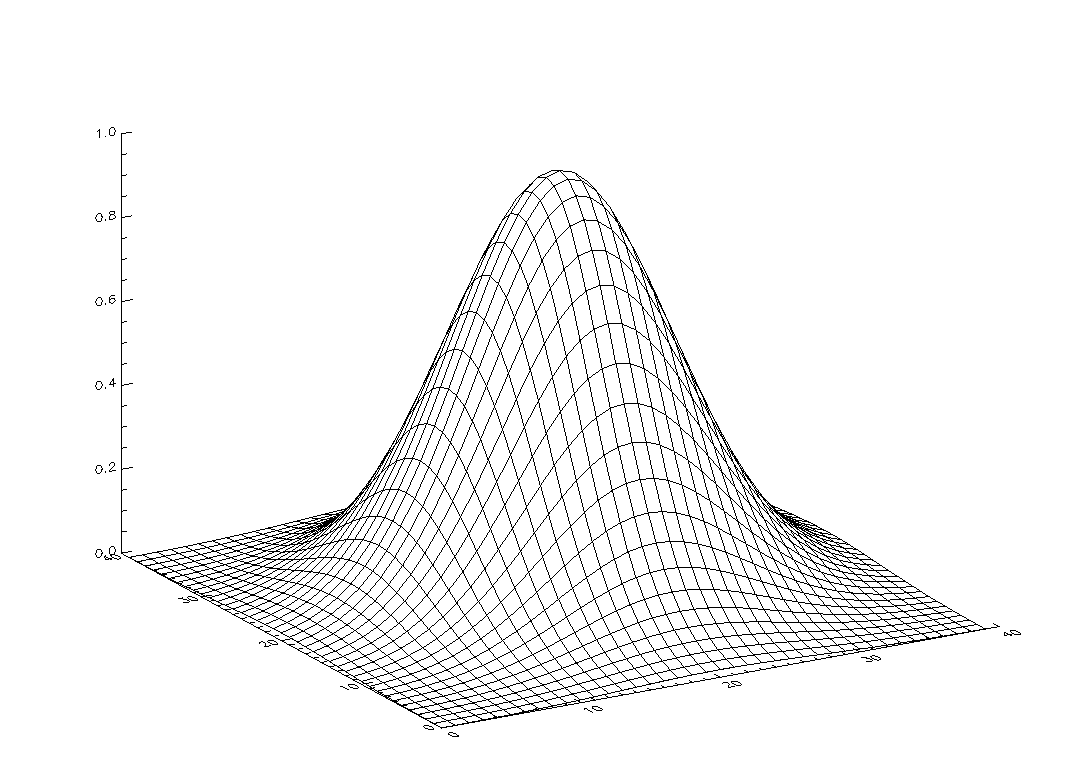
\includegraphics[width=.6\textwidth]{2dgaussian.ps}
\caption{A Gaussian. \label{gaussfig}}
%NOTE THAT LABELS WORK ON FIGURES, TOO!!!
%****NOTE ALSO**** THAT THE LABEL MUST BE ****WITHIN**** THE CAPTION!!!
\end{center}
\end{figure}

In addition to width, you can define height, angle, and scale.  If you
specify only width or height, the other dimension scales automatically.
If you specify both, you can stretch the image.  Angle rotates the image
by some number of degree in the positive direction. Scale multiplies the
picture's original size by the number you specify.
When specifying width or height, you must include units.  Some options
are: \verb$\$textwidth, in, cm, pt, em, ex. See the Not So Short Guide for more
info.

If you want to display several pictures together or have size scaling or
stretching or rotation, as in Figure \ref{silly}, you can do this.

\begin{figure} [!p]
%the [p!] tells latex you want the figure on a new page 
\begin{center}
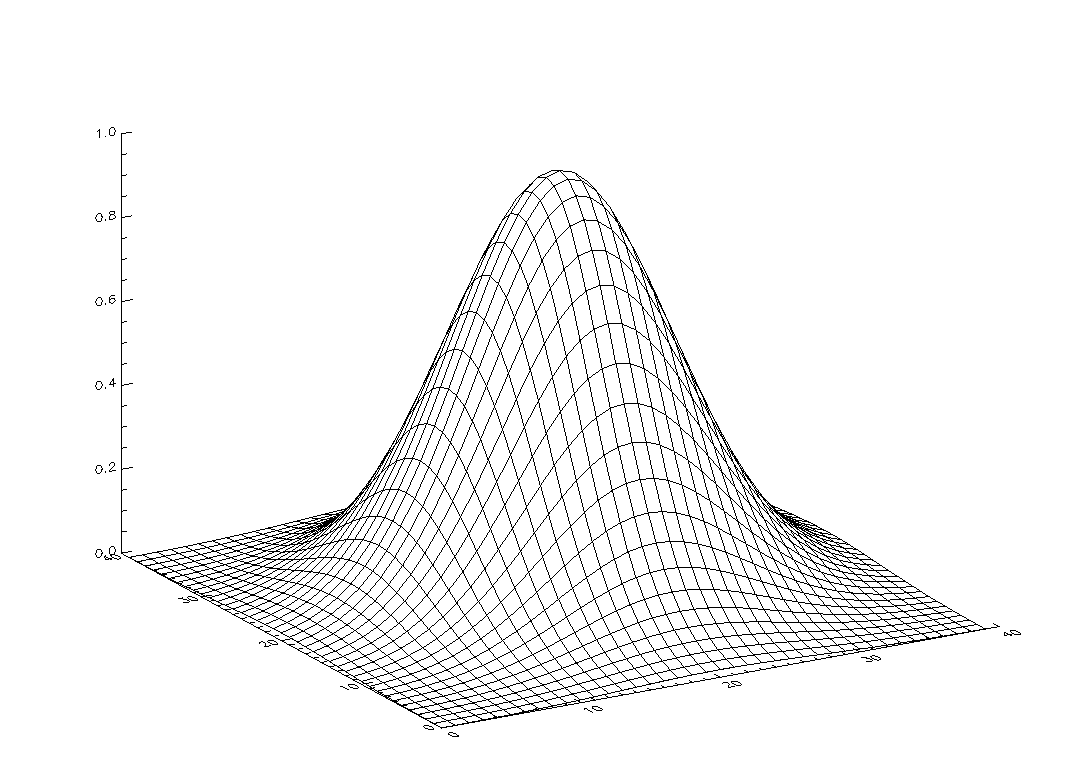
\includegraphics[width=1in,height=5in]{2dgaussian.ps}
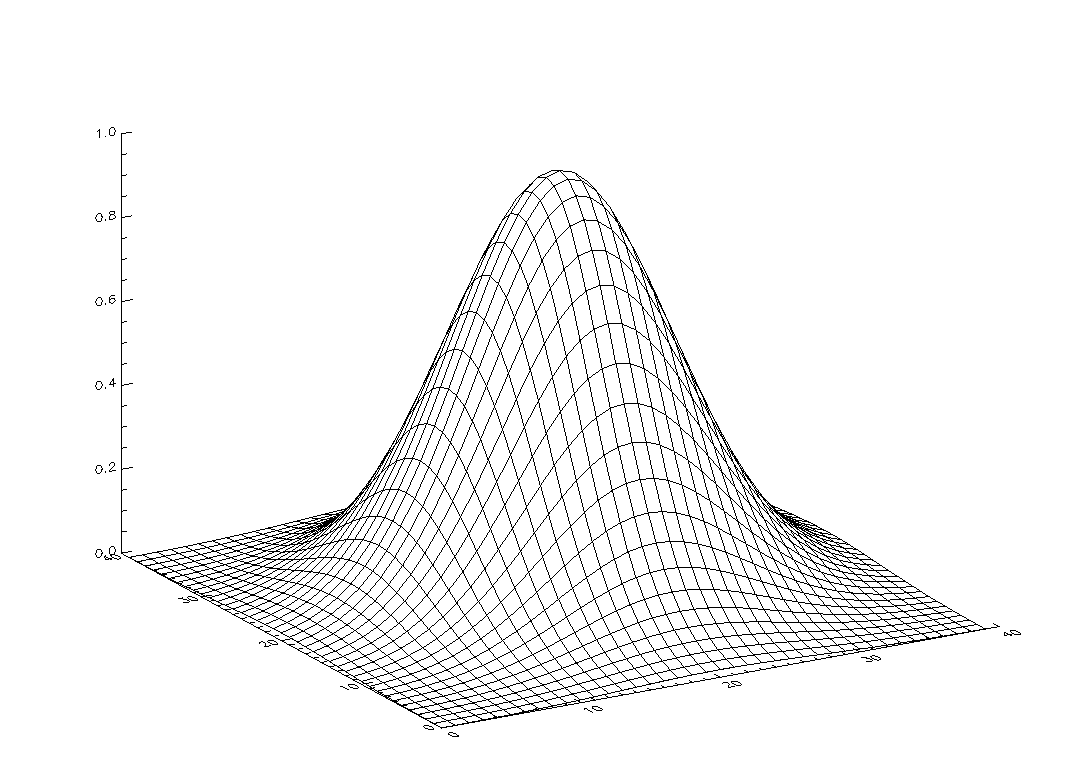
\includegraphics[width=5in,height=1in,angle=180]{2dgaussian.ps}
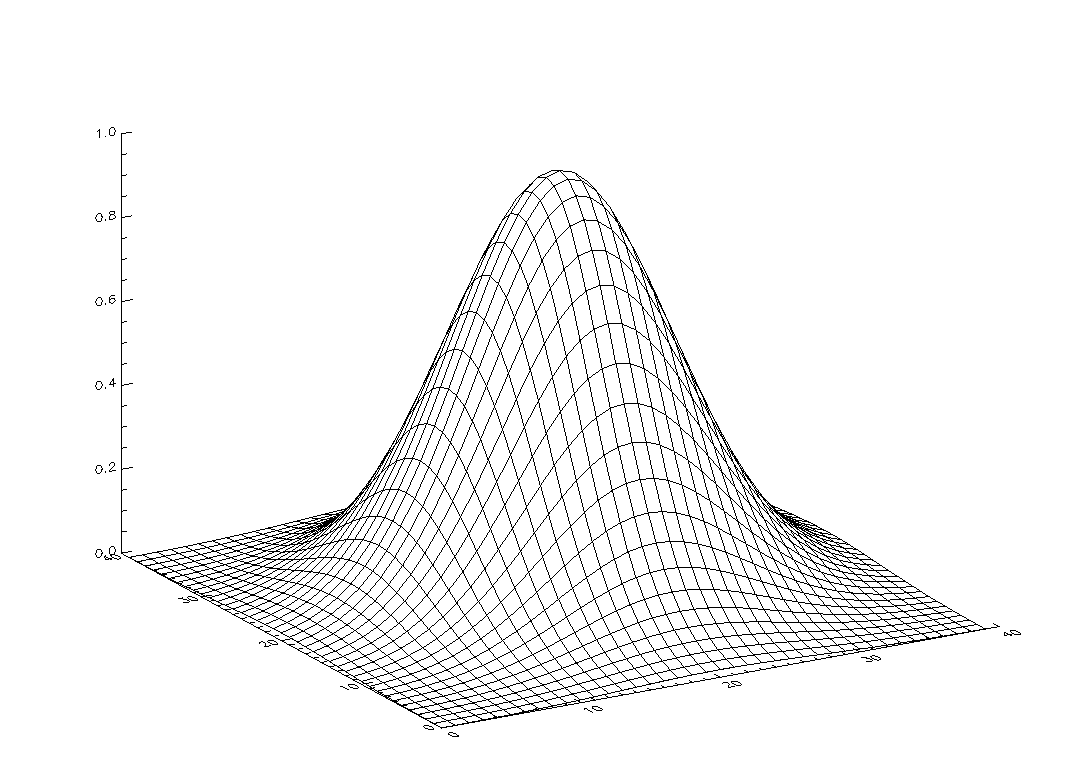
\includegraphics[scale=0.1,angle=45]{2dgaussian.ps}
\end{center}
\caption{This is a very silly figure! \label{silly}}
\end{figure}

	One of the most difficult tasks for the novice (and, even, the
experienced!) typesetter is image placement.  \LaTeX\ places floating
bodies where it thinks they best fit, which isn't always the most
logical place in a document. You have one way to control placement: the
placement commands, which work for tables and figures. They are: {\tt
[h!], [t!], [p!], [b!]}, meaning: ``put here'', ``put at top of page'',
''make a new page'', ``put at bottom of page''. We used {\tt [h!]} for
Figure \ref{gaussfig} and {\tt [p!]} for Figure \ref{silly}. Sometimes
they are frustratingly inattentive to your desires; this occurs because
\LaTeX\ is smarter than you think it is---there's not enough space to
put the figure exactly where you want it. .Judicious use of sizing (for
images) and using smaller fonts (for tables\footnote{To temporarily use
a smaller font: {\tt {\small [small text\dots]}}or even {\tt {\tiny
[tiny text\dots]}}}), or relocating, are your only options.

\section{Tables}\label{tablesec}

        Tables are useful for displaying a large number of results.
There are two environments provided for tables; \verb&{table}&, which is
a \LaTeX\ resident environment, and \verb&{deluxetable}&, which is an
AAS\TeX\ custom environment.   Table \ref{normtable} is the {\tt \{table\}}, a simpler
version for which the placement commands work; Table \ref{2abs} is the {\tt
deluxetable}, a more elaborate version for which the placement commands
do not work---it always puts the table at the very end, so it's not very
nice for lab reports.

\noindent Let's begin with the ordinary table, which is more flexible
because you the placement commands work; here we use {\tt [b!]},
specifying its location to be the bottom of the page\dots

\begin{table}[!b]
%THE [!b] TELLS IT TO PUT THE TABLE AT THE BOTTOM OF THE PAGE. 
%IF YOU USED [!t] IT WOULD PUT IT AT THE TOP.
\begin{center}
\caption{Sample table \label{normtable}}
%TABULAR FORMAT IS THE WORD HERE; the c's represent centered
%columns, and the vertical bars represent vertical lines. 
%Lines are broken by \\, and columns are separated by the
%ampersand.
\begin{tabular}{|c|c|} \hline
Temperature & Voltage Drop \\
\hline
\hline
310K & 0.6761V$\pm$0.0004V\\
\hline
300K & 0.7064V$\pm$0.0005V\\
\hline
77K & 1.5318V$\pm$0.001V\\
\hline
\end{tabular}
\end{center}
\end{table}

\clearpage
%NOTE THAT ONE CAN BREAK THE PAGE BY USING \clearpage....

\noindent And now, we end with the deluxetable; it's always at the end, on
its very own page. Because we're ending with it, this is one of the few
instances where it's properly placed---but because it's on its own page,
it's placement definitely not elegant!

\begin{deluxetable}{crrcrrl} %the crrrl's set text alignment
%[AOWING TO VARIOUS PECULIARITIES, YOU SHOULD HAVE NO BLANK LINES INSIDE
%THE DELUXETABLE ENVIRONMENT--IN CONTRAST TO ALL OTHER PLACES IN TEX.
\footnotesize
\tablecaption{Sample table \label{2abs}}
\tablewidth{0pt}
\tablehead{
\colhead{Source} & \colhead{$\ell$} & \colhead{$b$} &
\colhead{$\tau_{max}$} &
\colhead{$v_{LSR}$} & \colhead{FWHM} & \colhead{ref, note}
}
\startdata
0624-058 (3C161) & 215.4 & --8.0  &    0.67      &  12.0 &   4.5 &   1,a
\\
3C161            & 215.4 & --8.0  &   0.88       &   7.6 &   2.5 &   1,a
\\
3C161(OH)        & 215.4 & --8.0  &  0.013       &   8.6 &   1.2 &   3
\\
PKS0605-08       & 215.7 & --13.5 &
0.80$^b$         &  7.3  &   8.9 &   2
\\
0530+04 (4C04.18)& 200.0 & --15.3 & 0.8:         &  4.3: &   6.7:&   2
\\
3C135            & 200.5 & --21.0 & $\lesssim 0.11$&\nodata &\nodata & 2
\\
PKS0533-12       & 215.4 & --22.2 & 0.36         &  3.9  &   8.0 &    2
\\
\enddata
\tablerefs{(1) Mebold {\it et al.} (1981), Mebold
{\it et al.} (1982); (2) Crovisier, Kaz\`es, and Aubrey (1978);
(3) Dickey, Crovisier, and Kaz\`es (1981).}
\tablenotetext{a}{Mebold {\it et al.} (1982) list 3 components in
addition to the 4 listed here.}
\tablenotetext{b}{We have not listed a second, weaker Gaussian component
because of poor signal/noise.}
\tablecomments{This comment applies to the whole table and you can
put it either in front or behind the other comments.}
\end{deluxetable}

\end{document}

Note that anything here is skipped by the interpretor.  You can use it
as scratch paper or to keep templates handy when working on a document. 
Alternately, if you're trying to fix a document with a whole bunch of
bugs in it, temporarily tossing a \end{document} in the middle of the
file will save time, since the compiler won't bother trying to decipher
problems.

